\begin{exo}
	Un jeu de domino est composé des pièces ci-dessous. On retourne les dominos, on les mélange et on en choisit un au hasard.

	\begin{center}
		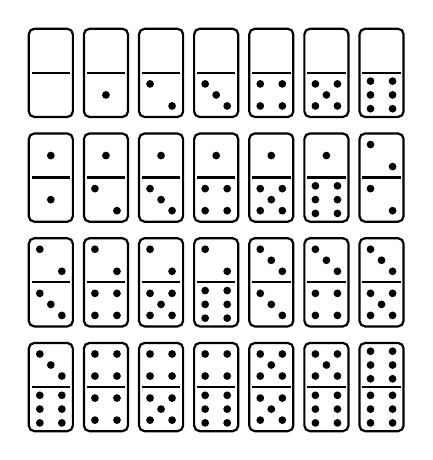
\begin{tikzpicture}[scale=0.35]
			\def\domino#1#2{
				\draw[rounded corners=2pt, thick, fill=white] (-0.8,-1.6) rectangle (0.8,1.6);
				\draw[thick] (-0.7,0) -- (0.7,0);
				\ifnum#1=1 \fill (0,0.8) circle (4pt); \fi
				\ifnum#1=2 \fill (-0.4,1.2) circle (4pt); \fill (0.4,0.4) circle (4pt); \fi
				\ifnum#1=3 \fill (-0.4,1.2) circle (4pt); \fill (0,0.8) circle (4pt); \fill (0.4,0.4) circle (4pt); \fi
				\ifnum#1=4 \fill (-0.4,1.2) circle (4pt); \fill (0.4,1.2) circle (4pt); \fill (-0.4,0.4) circle (4pt); \fill (0.4,0.4) circle (4pt); \fi
				\ifnum#1=5 \fill (-0.4,1.2) circle (4pt); \fill (0.4,1.2) circle (4pt); \fill (0,0.8) circle (4pt); \fill (-0.4,0.4) circle (4pt); \fill (0.4,0.4) circle (4pt); \fi
				\ifnum#1=6 \fill (-0.4,1.3) circle (4pt); \fill (-0.4,0.8) circle (4pt); \fill (-0.4,0.3) circle (4pt); \fill (0.4,1.3) circle (4pt); \fill (0.4,0.8) circle (4pt); \fill (0.4,0.3) circle (4pt); \fi
				\ifnum#2=1 \fill (0,-0.8) circle (4pt); \fi
				\ifnum#2=2 \fill (-0.4,-0.4) circle (4pt); \fill (0.4,-1.2) circle (4pt); \fi
				\ifnum#2=3 \fill (-0.4,-0.4) circle (4pt); \fill (0,-0.8) circle (4pt); \fill (0.4,-1.2) circle (4pt); \fi
				\ifnum#2=4 \fill (-0.4,-0.4) circle (4pt); \fill (0.4,-0.4) circle (4pt); \fill (-0.4,-1.2) circle (4pt); \fill (0.4,-1.2) circle (4pt); \fi
				\ifnum#2=5 \fill (-0.4,-0.4) circle (4pt); \fill (0.4,-0.4) circle (4pt); \fill (0,-0.8) circle (4pt); \fill (-0.4,-1.2) circle (4pt); \fill (0.4,-1.2) circle (4pt); \fi
				\ifnum#2=6 \fill (-0.4,-0.3) circle (4pt); \fill (-0.4,-0.8) circle (4pt); \fill (-0.4,-1.3) circle (4pt); \fill (0.4,-0.3) circle (4pt); \fill (0.4,-0.8) circle (4pt); \fill (0.4,-1.3) circle (4pt); \fi
			}
			\begin{scope}[shift={(0,0)}]\domino{0}{0}\end{scope}
			\begin{scope}[shift={(2,0)}]\domino{0}{1}\end{scope}
			\begin{scope}[shift={(4,0)}]\domino{0}{2}\end{scope}
			\begin{scope}[shift={(6,0)}]\domino{0}{3}\end{scope}
			\begin{scope}[shift={(8,0)}]\domino{0}{4}\end{scope}
			\begin{scope}[shift={(10,0)}]\domino{0}{5}\end{scope}
			\begin{scope}[shift={(12,0)}]\domino{0}{6}\end{scope}
			\begin{scope}[shift={(0,-3.8)}]\domino{1}{1}\end{scope}
			\begin{scope}[shift={(2,-3.8)}]\domino{1}{2}\end{scope}
			\begin{scope}[shift={(4,-3.8)}]\domino{1}{3}\end{scope}
			\begin{scope}[shift={(6,-3.8)}]\domino{1}{4}\end{scope}
			\begin{scope}[shift={(8,-3.8)}]\domino{1}{5}\end{scope}
			\begin{scope}[shift={(10,-3.8)}]\domino{1}{6}\end{scope}
			\begin{scope}[shift={(12,-3.8)}]\domino{2}{2}\end{scope}
			\begin{scope}[shift={(0,-7.6)}]\domino{2}{3}\end{scope}
			\begin{scope}[shift={(2,-7.6)}]\domino{2}{4}\end{scope}
			\begin{scope}[shift={(4,-7.6)}]\domino{2}{5}\end{scope}
			\begin{scope}[shift={(6,-7.6)}]\domino{2}{6}\end{scope}
			\begin{scope}[shift={(8,-7.6)}]\domino{3}{3}\end{scope}
			\begin{scope}[shift={(10,-7.6)}]\domino{3}{4}\end{scope}
			\begin{scope}[shift={(12,-7.6)}]\domino{3}{5}\end{scope}
			\begin{scope}[shift={(0,-11.4)}]\domino{3}{6}\end{scope}
			\begin{scope}[shift={(2,-11.4)}]\domino{4}{4}\end{scope}
			\begin{scope}[shift={(4,-11.4)}]\domino{4}{5}\end{scope}
			\begin{scope}[shift={(6,-11.4)}]\domino{4}{6}\end{scope}
			\begin{scope}[shift={(8,-11.4)}]\domino{5}{5}\end{scope}
			\begin{scope}[shift={(10,-11.4)}]\domino{5}{6}\end{scope}
			\begin{scope}[shift={(12,-11.4)}]\domino{6}{6}\end{scope}
		\end{tikzpicture}
	\end{center}
	\begin{enumerate}
		\item Quelle est la probabilité d'obtenir un double ?
		\item En déduire la probabilité de ne pas obtenir un double.
		\item Quelle est la probabilité que la somme des points est inférieure ou égale à $6$ ?
	\end{enumerate}
\end{exo}
